\documentclass[a4paper,12pt]{article}
\usepackage{graphicx}
\usepackage[margin=0.3in]{geometry}

% Default fixed font does not support bold face
\DeclareFixedFont{\ttb}{T1}{txtt}{bx}{n}{12} % for bold
\DeclareFixedFont{\ttm}{T1}{txtt}{m}{n}{12}  % for normal

% Custom colors
\usepackage{color}
\definecolor{deepblue}{rgb}{0,0,0.5}
\definecolor{deepred}{rgb}{0.6,0,0}
\definecolor{deepgreen}{rgb}{0,0.5,0}
\definecolor{green}{rgb}{0,0.8,0}

% Python style for highlighting
\usepackage{listings}
\newcommand\pythonstyle{\lstset{
language=Python,
basicstyle=\ttm,
otherkeywords={self},             % Add keywords here
keywordstyle=\ttb\color{deepblue},
emph={MyClass,__init__},          % Custom highlighting
emphstyle=\ttb\color{deepred},    % Custom highlighting style
stringstyle=\color{deepgreen},
commentstyle=\color{green},
frame=tb,                         % Any extra options here
showstringspaces=false            % 
}}

% Python environment
\lstnewenvironment{python}[1][]
{
\pythonstyle
\lstset{#1}
}
{}

% Python for external files
\newcommand\pythonexternal[2][]{{
\pythonstyle
\lstinputlisting[#1]{#2}}}

% Python for inline
\newcommand\pythoninline[1]{{\pythonstyle\lstinline!#1!}}

\begin{document}

\section{MFT series expansion of the Ising model}
%\lstinputlisting[language=Python]{../random_walk.py}
\pythonexternal{../ising.py}

\begin{figure}[h]
    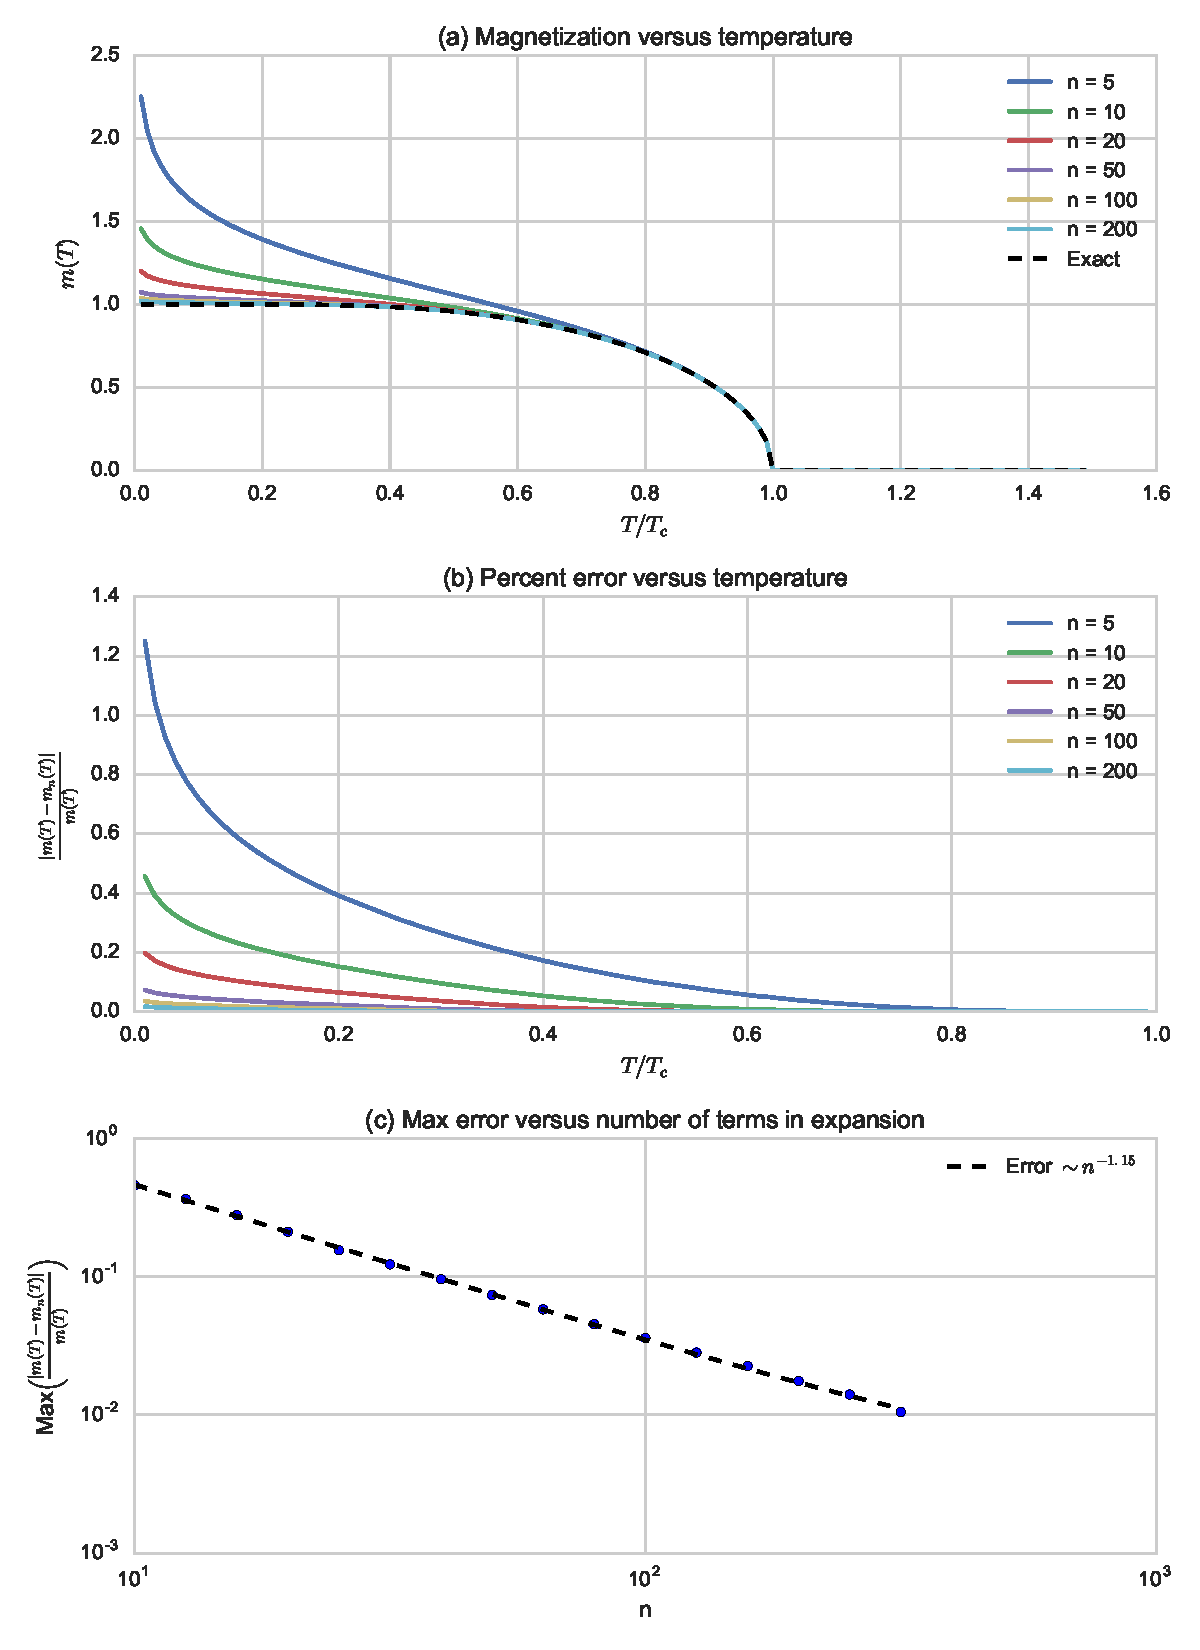
\includegraphics[width=\linewidth]{../ising.pdf}
\end{figure}

\noindent The figure produced by the above code is on the next page.

When approximating the Ising magnetization, the largest deviation from the exact solution occurs at low values of $T$, as can be seen in (a) and (b). To determine the required number of terms $n$ to reach agreement within 1\%, the maximum error was computed at values ranging from $n$ = 10 to 1000, but ended prematurely around $n \approx 300$ due to an overflow error ($m^n$ terms being the culprit). Fortunately, this is also around the number of terms required to be within 1\% of the exact solution. Additionally, the error was found to scale as approximately $n^{-1.15}$.
\end{document}
